\begin{figure}[ht]
\centering
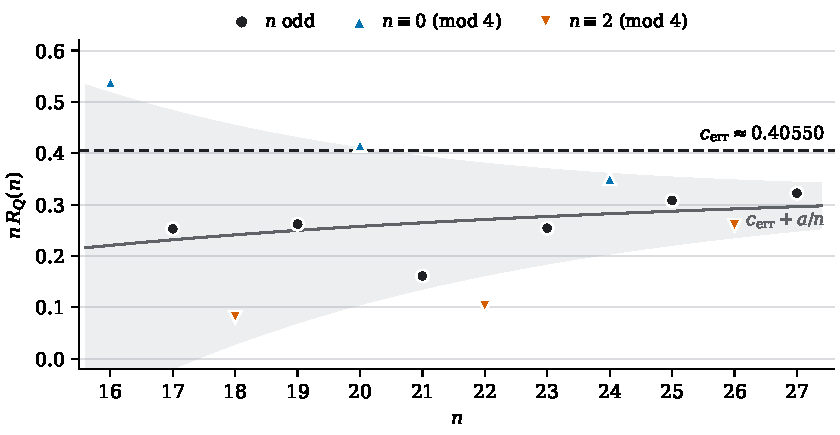
\includegraphics[width=.9\linewidth]{figuras/conteos.pdf}
\caption{Values of $nR_Q(n)$ for $16\le n\le27$, obtained from the exact counts and the canonical
predictor (numerical evidence). The dashed line marks the estimate of $\cerr$. The gray curve shows
the fitted drift $\cerr+a/n$, with $a\simeq-2.956$, and the shaded band has the amplitude
$Ae^{-\kappa(n-16)}$ of the period-four oscillation (Appendix~\ref{app:numquad}). The odd sizes lie
near the drift. Multiples of four lie above it, and those that leave remainder two when divided by
four lie below it.}\label{fig:counts}
\end{figure}
